\documentclass[]{llncs}

\usepackage{amsmath}
\usepackage{graphicx}
\usepackage{float}
\usepackage{color, colortbl}
\usepackage{xcolor}

\begin{document}

\title{Collision-Free WLANs: From Concepts to Working Protocols. A PhD. Proposal}
\author{Luis Sanabria-Russo}
\institute{Universitat Pompeu Fabra, Barcelona Spain \\ \email{luis.sanabria@upf.edu}}
\maketitle

\begin{abstract}
In the upcoming years the number of devices that exchange data wirelessly is though to increase dramatically, even nowadays home environments no longer lack the wireless network congestion only seen before at office/public spaces (like wireless hot-spots). The current Medium Access Control (MAC) protocol is known to be prone to collisions, which increase with the number of stations in the wireless network. Many proposals have been made to amend the current standard, but at the time of this writing the drawbacks related to collisions have not been fixed. One of the reasons why implementing new MAC protocols is a challenging task relates to the need for really fast processing speed (which can only be achieved at hardware level) and the need for more realistic channel conditions and traffic scenarios.

This PhD Thesis Proposal aims at designing and prototyping next-generation MAC protocols for IEEE 802.11-like networks, going from concept proposals to hardware implementation.

% These challenges reveal the need for collision-free medium access control protocols capable of allocating large number of stations that are foreseeable in the future of wireless local area networks. Furt


% The current standard for medium access control in Wireless Local Area Networks (WLANs) called Carrier Sense Multiple Access with Collision Avoidance (CSMA/CA), is by its nature prone to collisions. These happen as a consequence of randomizing the backoff counter each contender must select in order to coordinate its transmissions. Carrier Sense Multiple Access with Enhanced Collision Avoidance (CSMA/ECA) introduces minor adjustments to CSMA/CA  that eliminate the possibility of collisions after a short convergence period. Its principle is to select a deterministic backoff after successful transmissions instead of a random one (as in CSMA/CA), allowing contenders to \emph{own} a time slot in the schedule. 
\end{abstract}

\section{Introduction}\label{introduction}
	Carrier Sense Multiple Access with Collision Avoidance (CSMA/CA) is the protocol used in Wireless Local Area Networks (WLANs) to coordinate transmissions. Nodes should avoid simultaneous transmissions because the medium is shared, so concurrent transmissions attempts will result in indecipherable messages to the receivers. This event is referred to as a \emph{collision}. 

For CSMA/CA, time is slotted. As a result, there are three kind of slots: \emph{empty}, \emph{successful} and \emph{colllision} slots, where successful and collision slots contain successful transmissions or collision events. While the remaining are just tiny empty slots of a fixed time length.

Every time there is a contention for transmission, CSMA/CA forces contenders to count down from a randomly generated number (from now on referred to as backoff counter), decrementing it by one per every passing empty slot. When the backoff expires (reaches zero), contenders will attempt transmission. Nevertheless, because the backoff counter is generated at random, there might be cases where two or more contenders simultaneously attempt transmission and a collision occurs, significantly degrading the throughput of the system.

It is possible to obtain greater levels of throughput than the achieved by CSMA/CA under optimal parameter configuration by picking a deterministic backoff counter after successful transmissions. This approach is called Carrier Sense Multiple Access with Enhanced Collision Avoidance (CSMA/ECA)~\cite{CSMA_ECA}. Results also show that by making simple modifications on the behavior of the current protocol, CSMA/ECA is able to allocate more contenders in a collision-free fashion while preserving the system fairness by equally distributing the system throughput among all nodes. 
% Furthermore, CSMA/ECA is resilient to synchronization flaws on the wireless network cards that can cause a miscount of passing slots (slot drift), as opposed to other MAC protocols~\cite{slotDrift}.
% 

Many years of testing have settled CSMA/CA as the default protocol for this type of networks, even-though many other proposals claim to outperform it, e.g.~\cite{CSMA_ECA,bellalta2009vtc,L_MAC2,HE,fairness-ECA}. Nevertheless, their proposed adjustments tested by simulation are not included in the current standard.

Recent approaches to design and implement MAC protocols on cheap commodity hardware~\cite{WMP,FLAVIA} opened the possibility to prototype some of the protocols proposed by the research community. Although at an early phase and steep learning curve, these alternatives allow researchers of all levels to make substantial contributions.

\subsection{Motivation}\label{motivation}
As mentioned before, many proposals to amend the collision problem in CSMA/CA have been made and none is included in the current standard.

Taking a guess-look at what is to come in a few years time, WLANs are expected to be as crowded as never before. From tablets, laptops, smart phones, watches, smart health/activity monitoring devices; to traffic prioritization, accommodating these many devices and services will soon out-challenge CSMA/CA.

Even-though CSMA/CA in theory is able to coordinate medium access for many contenders, it does so at the price of a reduced throughput induced by collisions. This is completely leveraged by CSMA/ECA, which in fact provides greater throughput than CSMA/CA in almost every testable scenario.

The goal of this PhD Thesis is twofold: $1$) further analyze CSMA/ECA behavior considering unsaturated scenarios, and $2$) to write the protocol into cheap commodity Wireless Network Interface Cards (WNICs) using the principles proposed in \cite{WMP}. The expected results from this work are the evaluation and testing in real hardware of a MAC protocol capable of allocating a large number of contenders in a collision-free fashion, ensuring long-term throughput fairness and able to comply with current quality of service (QoS) specifications for WLANs. 

This work is expected to collect enough evidence for the community to consider its contributions for upcoming amends to the standard. Furthermore, the progress reports and tools developed during the research effort will provide sufficient background for its replication and further development of MAC protocols in real hardware.



% The expected results from this work will provide a complete overview of CSMA/ECA and sufficient documentation to make an amendment proposal to CSMA/CA.
\section{State of the Art}\label{stateOfTheArt}
	For the following paragraphs, an overview of the state of the art is presented. Ranging from the current standard passing through other proposed protocols to end at the description of CSMA/ECA and the Wireless MAC Processor architecture~\cite{WMP}.

It is worthwhile to note that the words \emph{node}, \emph{contenders} and \emph{stations} may be used interchangeably without any different implication.

\subsection{CSMA/CA: the current standard}
Each node in a WLANs runs an instance of CSMA/CA protocol. As briefly mentioned in Section~\ref{introduction}, in this time-slotted networks nodes draw a random backoff counter $B\in[0,CW(k)]$ everytime they have a packet to transmit; where $CW(k)=2^{k}CW_{\min}$ is the contention window at backoff stage $k\in[0,m]$ with $m$ its maximum value, and $CW_{\min}$ being the minimum contention window.

Every passing empty slot decrements the backoff counter in one, and freezes when another node's transmission is detected. When the backoff expires ($B=0$), the contending node attempts transmission.

Because the backoff is computed at random, it is possible that two or more nodes pick the same value. When the corresponding stations attempt transmission, none will receive an \emph{ACKnowledgement} (ACK) from the receiver given that they attempted transmission at the same time. This is considered a collision.

The way CSMA/CA handles collisions is summarized in the following bullets:
\begin{itemize}
	\item A collision is assumed if no ACK is received by the transmitter.
	\item CSMA/CA instructs colliding nodes to double their contention window by increasing the backoff stage $k$ in one. This measure doubles the range of possible values drawn when computing the backoff counter, thus reducing the probability of two stations picking the same value.
\end{itemize}

If a node successfully transmits (receives an ACK from the receiver):
\begin{itemize}
	\item Resets its backoff stage ($k=0$).
	\item If it has another packet to transmit, the node generates a backoff counter and the process is restarted.
\end{itemize}

CSMA/CA uses a Binary Exponential Backoff (BEB) technique in order to reduce the collision probability (or the event of two stations picking the same backoff counter). Nevertheless, this technique does not eliminate collisions, in fact, stations that have successfully transmitted in the past may collide in the future. Figure~\ref{fig:csmaCA} provides and example of CSMA/CA's behavior.

\begin{figure}[htbp]
  \centering
  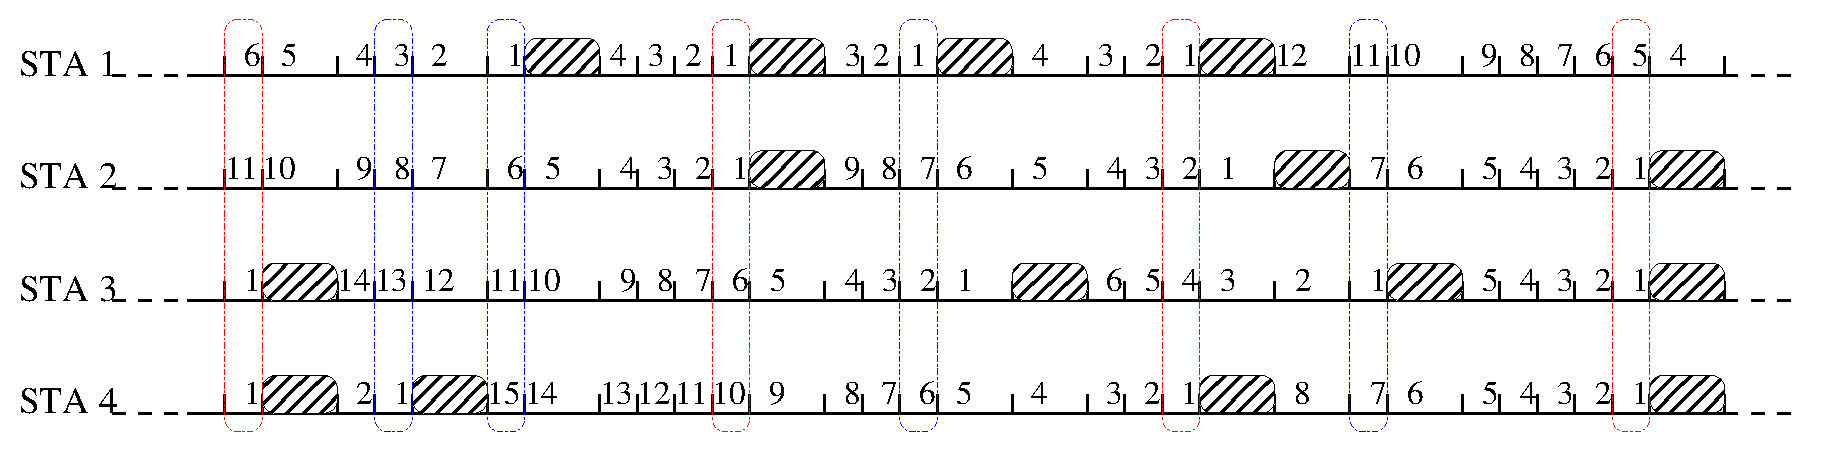
\includegraphics[width=\linewidth]{csma_ca_short.eps}
  \caption{For stations running CSMA/CA ($CW_{\min}=16$)
  \label{fig:csmaCA}}
\end{figure}

\subsection{Going beyond CSMA/CA's throughput}
There have been many works proposing modifications to CSMA/CA~\cite{CSMA_ECA,bellalta2009vtc,L_MAC2,HE,bharghavan1994map,wang2004ncr,cali2000dti,lopez-toledo2006aoi,barcelo2008lba,hui2011epp,barcelo2011tcf}. Nevertheless, and as pointed out in~\cite{research2standards}, there is a group among them that considers backwards compatibility with legacy users and at the same time provides levels of throughput beyond those provided by CSMA/CA.

The increase in throughput is the result of choosing a deterministic backoff counter instead of a random one. This approach was first introduced in~\cite{barcelo2008lba} and then tested under different conditions such as saturated and unsaturated scenarios~\cite{CSMA_ECA,bellalta2009vtc,L_MAC2,HE}. It is called Carrier Sense Multiple Access with Enhanced Collision Avoidance (CSMA/ECA) and its similarities and differences with CSMA/CA are described in the following.

CSMA/ECA is a collision-free MAC protocol that allows many contenders to coordinate access to the medium in a totally distributed manner. It starts from the simple idea of picking a deterministic backoff counter $B_{d}=CW(k)/2$ after successful transmissions. By doing so, nodes that successfully transmitted in the past, will do so without colliding with other CSMA/ECA nodes in future cycles. Hence the collision-free state.

Nevertheless, when the number of contenders ($n$) is greater than the deterministic backoff ($n>B_{d}$), collisions reappear. CSMA/ECA handles collision much more like CSMA/CA does, but in order to restore the collision-free state with this increased number of contenders, CSMA/ECA instructs nodes {\bfseries not} to reset their backoff stage ($k$), resulting in a increased $B_{d}$. This is called \emph{Hysteresis}, and ensures that many more contenders can be allocated in a collision-free state.

Hysteresis instructs some nodes to have greater backoff counters than others, unevenly sharing channel access time. This unfairness issue is leveraged by instructing nodes at backoff stage $k$ to transmit $2^{k}$ packets on each attempt, thus proportionally compensating those nodes at higher backoff stages. This measure was first proposed by Fang et al.~\cite{L_MAC2}, and further implemented as \emph{Fair Share}~\cite{research2standards} for CSMA/ECA. Figure~\ref{fig:csmaECA} shows and working example of CSMA/ECA.

\begin{figure}[htbp]
  \centering
  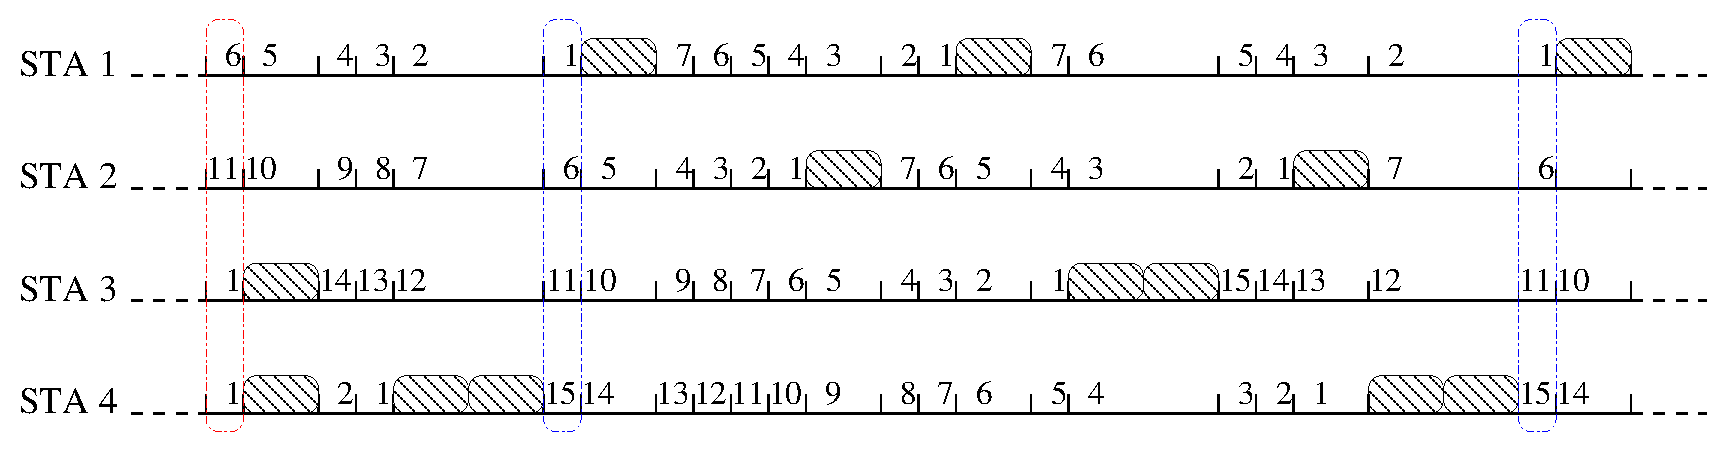
\includegraphics[width=\linewidth]{csma_eca_different_backoff_short.eps}
  \caption{For stations running CSMA/ECA ($CW_{\min}=16$)
  \label{fig:csmaECA}}
\end{figure}

\subsection{Prototyping MAC protocols in real hardware}
MAC protocols face new challenges that come alongside upcoming scenarios, like: vehicular, mesh and ad-hoc networks; quality of service (QoS) and traffic differentiation; spectrum reutilization in cognitive networks. 

Although many proposals address the shortcomings of the current protocol in these upcoming scenarios, many are discarded either for deviating too much from the current standard operation or for their unlikeliness of real-world deployment when time-critical tasks are modified.

The current implementation of MAC protocols in WNICs is done in a closed form, meaning that usually time-critical (or Lower-MAC) tasks are hardware-coded without the possibility of modification by third-parties.

One step towards openness came with the release of OpenFWWF~\cite{OpenFWWF}, the first open-source firmware of the Distributed Coordination Function (DCF) that rules CSMA/CA operation in WLANs. Its release opened the possibility for modifications to the Lower-MAC, thus augmenting its potential against other slower options like the ones using the Universal Software Radio Peripheral (USRP)~\cite{ettus2008universal} and GNURadio~\cite{blossom2004gnu} combination~\cite{tan2011sora} or the still hardware-limited FPGA alternatives, like~\cite{ng2010airblue}.

Nevertheless, OpenFWWF is tightly related to the hardware platform it was released for (Broadcom/AirForce54G cards) and extensions require rewriting of large chunks of assembly code, which makes it difficult to implement by non-experts.

Wireless MAC Processors (WMP)~\cite{WMP} aim at lowering the barriers for MAC protocol implementation in commodity hardware. By carefully identifying and translating the MAC operations into different Extended Finite State Machines (XFSM), it became possible to designate Lower-MAC tasks to the general-purpose CPU equipped in most WNICs. Furthermore, the WMP-Editor (shown in Figure~\ref{fig:WMPEditor}) allows programmers to combine different XFSM and configure the MAC events and conditions that would trigger their tasks.

% and allow programmers to decide when those tasks ought to be performed (based on events and/or conditions). 

\begin{figure}[htbp]
  \centering
  \includegraphics[width=\linewidth]{WMP-EditorLayout.eps}
  \caption{WMP-Editor Layout
  \label{fig:WMPEditor}}
\end{figure}

\bibliographystyle{splncs}
\bibliography{ref}

\end{document}

